% \documentclass[aspectratio=169,notes]{beamer}
\documentclass[aspectratio=169]{beamer}
\usetheme[faculty=phil]{fibeamer}
\usepackage{polyglossia}
\setmainlanguage{english} %% main locale instead of `english`, you
%% can typeset the presentation in either Czech or Slovak,
%% respectively.
\setotherlanguages{russian} %% The additional keys allow
%%
%%   \begin{otherlanguage}{czech}   ... \end{otherlanguage}
%%   \begin{otherlanguage}{slovak}  ... \end{otherlanguage}
%%
%% These macros specify information about the presentation
\title[Theoretical Mechanics]{Week HW 7, KIN ENERGY NEWTON EULER} %% that will be typeset on the
\subtitle{Theorem on the Change of Kinetic Energy of a System\\
Newton-Euler equation\\
\ 
         } %% title page.
\author{Oleg Bulichev}
%% These additional packages are used within the document:
\usepackage{ragged2e}  % `\justifying` text
\usepackage{booktabs}  % Tables
\usepackage{tabularx}
\usepackage{tikz}      % Diagrams
\usetikzlibrary{calc, shapes, backgrounds}
\usepackage{amsmath, amssymb}
\usepackage{url}       % `\url`s
\usepackage{listings}  % Code listings
% \usepackage{subfigure}
\usepackage{floatrow}
\usepackage{subcaption}
\usepackage{mathtools}
\usepackage{todonotes}
\usepackage{fontspec}
\usepackage{multicol}
\usepackage{pdfpages}
\usepackage{wrapfig}
\usepackage{animate}
\usepackage{booktabs}
\usepackage{multirow}
% \usepackage{graphicx}
\usepackage{colortbl}

\graphicspath{{resources/}}
\frenchspacing

\setbeamertemplate{caption}[numbered]
\usetikzlibrary{graphs}

% \usepackage[backend=biber,style=ieee,autocite=footnote]{biblatex}
% \addbibresource{biblio.bib}
% \DefineBibliographyStrings{english}{%
%   bibliography = {References},}

\newcommand{\oleg}[2][] {\todo[color=red, #1] {OLEG:\\ #2}}
\newcommand{\fbckg}[1]{\usebackgroundtemplate{\includegraphics[width=\paperwidth]{#1}}}%frame background

\usepackage[framemethod=TikZ]{mdframed}
\newcommand{\dbox}[1]{
\begin{mdframed}[roundcorner=3pt, backgroundcolor=yellow, linewidth=0]
\vspace{1mm}
{#1}
\vspace{1mm}
\end{mdframed}
}

\begin{document}
\setlength{\abovedisplayskip}{0pt}
\setlength{\belowdisplayskip}{0pt}
\setlength{\abovedisplayshortskip}{0pt}
\setlength{\belowdisplayshortskip}{0pt}

\fbckg{fibeamer/figs/title_page.png}
\frame[c]{\setcounter{framenumber}{0}
    \usebeamerfont{title}%
    \usebeamercolor[fg]{title}%
    \begin{minipage}[b][6.5\baselineskip][b]{\textwidth}%
        \textcolor{black}{\raggedright\inserttitle}
    \end{minipage}
    % \vskip-1.5\baselineskip

    \usebeamerfont{subtitle}%
    \usebeamercolor[fg]{framesubtitle}%
    \begin{minipage}[b][3\baselineskip][b]{\textwidth}
        \raggedright%
        \insertsubtitle%
    \end{minipage}
    \vskip.25\baselineskip
}
%   \frame[c]{\maketitle}

\fbckg{fibeamer/figs/common.png}


\begin{frame}[t]{Task 1}
  \scriptsize
    \begin{minipage}{0.65\textwidth}
      A step ladder $ABC$, hinged at $B$, rests on a smooth horizontal floor, as shown on the figure. $AB=BC=2l$.
  
      The centres of gravity are at the midpoints $D$ and $E$ of the rods. The radius of gyration of each part of the ladder about the axis passing through the center of gravity is $p$.
  
      The distance between $B$ and the floor is $h$. At the certain moment the ladder collapses due to the rupture of a ling $FG$ between the two halves of the ladder. Neglecting the effect of friction in the hinge, determine:
      \begin{enumerate}
          \item the velocity $v_1$ of the point $B$ at the moment, when it hits the floor;
          \item the velocity $v_2$ of point $B$ at the moment, when it is at a distance $\dfrac{1}{2}h$ from the floor.
      \end{enumerate}
      \smallskip
  
      \textit{Answer}: $v_1=2l\sqrt{\dfrac{gh}{l^2+p^2}}$, $v_2 = \dfrac{1}{2}\sqrt{gh\dfrac{16l^2-h^2}{2(l^2+p^2)}}$.
    \end{minipage}
    \begin{minipage}{0.34\textwidth}
      \begin{figure}[H]
        \centering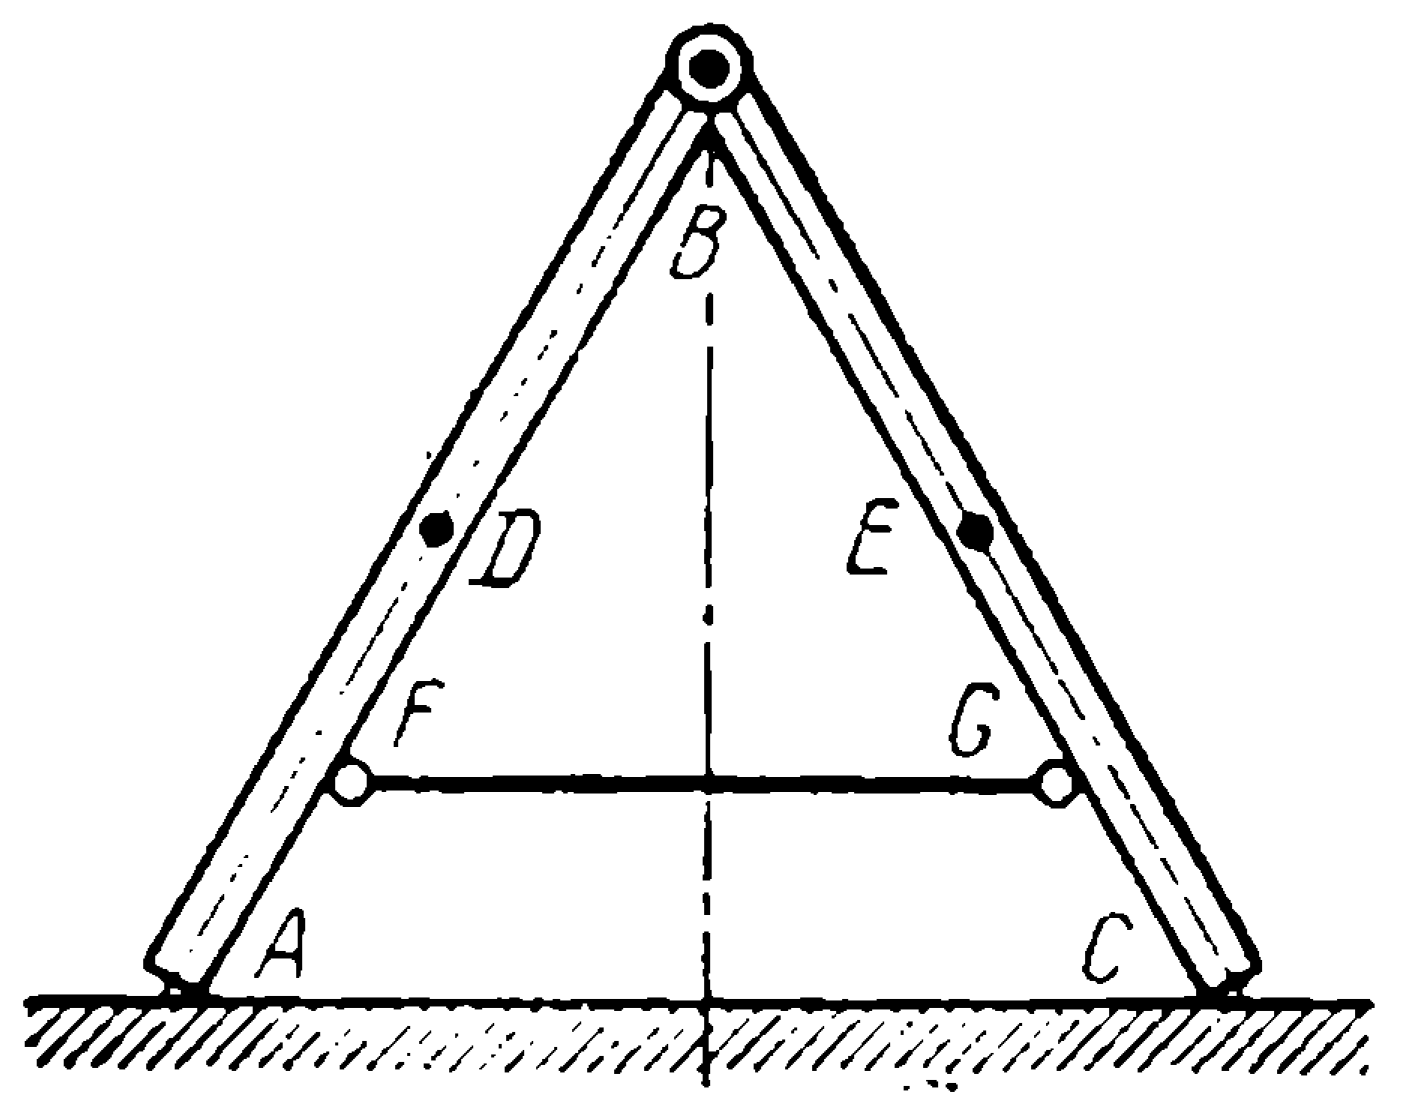
\includegraphics[height=6cm,width=1\textwidth,keepaspectratio]{HW7_1}
        \caption*{Task 1}
      \end{figure}
    \end{minipage}
  \end{frame}

  \begin{frame}[t]{Task 2 (Coding)}
  \framesubtitle{System description}
  \vspace{-0.6cm}
    \begin{columns}[T,onlytextwidth]
      \begin{column}{0.64\textwidth}
        \footnotesize
        You have a a cart pole. Body $1$ is a slider, mass $m_1$, it moves without friction.

        $AB$ is a massless rod with length $l$. Body $2$ with mass $m_2$ is connected to $AB$ in point $B$.
        \medskip

        It's a 2 DoF system. You should take $x$ and $\phi$ as a representation of this system. The origin of each coordinate should be the same as on the picture.
        \medskip

        Initial conditions:
        \begin{enumerate}
          \item $x = 0,\ \phi = 10^\circ,\ \dot{x} = 0,\ \dot{\phi} = 0,\ t=0$;
          \item $x = 0.5,\ \phi = 45^\circ,\ \dot{x} = 0,\ \dot{\phi} = 0,\ t=0$;
          \item $x = 0.5,\ \phi = -135^\circ,\ \dot{x} = 0,\ \dot{\phi} = 0,\ t=0$;
        \end{enumerate}
        Parameters: $m_1 = 5\ kg,\ m_2 = 1\ kg,\ l = 1\ m$.

      \end{column}
      \begin{column}{0.34\textwidth}
        \begin{figure}[H]
          \centering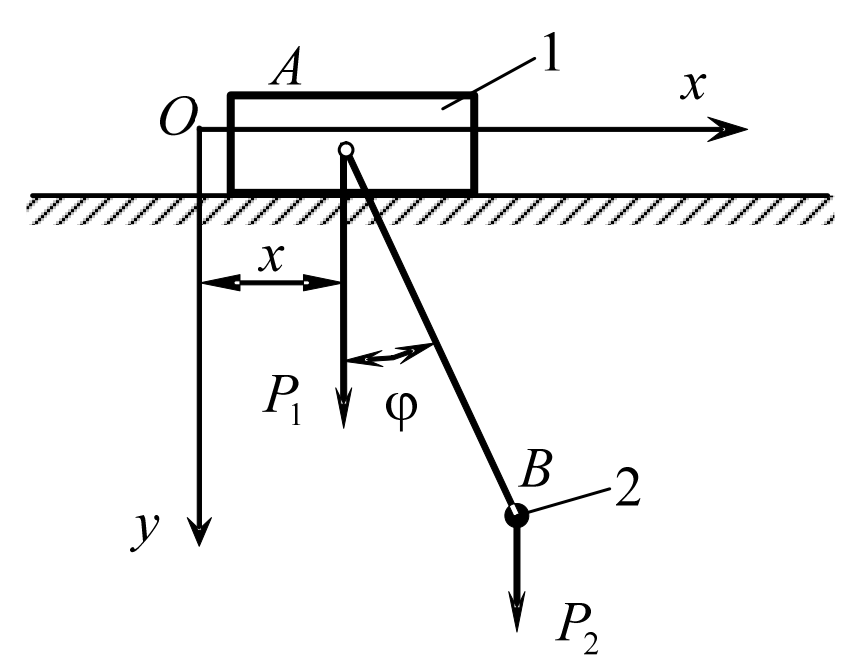
\includegraphics[height=6cm,width=1\textwidth,keepaspectratio]{HW7_2.png}
          \caption*{Task 2}
          \label{fig:HW7_2.png}
        \end{figure}
      \end{column}
    \end{columns}
  \end{frame}

  \begin{frame}[t]{Task 2 (Coding)}
    \framesubtitle{Tasks description}
          \footnotesize
          \vspace{-0.4cm}
          You should solve this problem using:
          \begin{enumerate}
            \item \textbf{Newton-Euler} method;
            \item Model-oriented design applications (\textit{SimInTech}, or MATLAB Simulink).
          \end{enumerate}
          \textbf{Tasks}
          \begin{enumerate}
            \item To derive a differential equation of the motion, using \textbf{Newton-Euler} approach.
            \item To create plots $x(t),\ \phi(t), \dot{x}(t), \dot{\phi}(t)$. 
            \item To make a simulation of this system. Show velocities and accelerations for $1,\ 2$ bodies (coding approach).
          \end{enumerate}
          \textbf{Artifacts}
          \begin{enumerate}
            \item Report in \textit{.pdf} or in \textit{.md}.
            \item For \textbf{Newton-Euler} method --- code, GIFs, plots.
            \item For \textbf{SimInTech} --- \textit{.prt}, for \textbf{Simulink} --- \textit{.slx} file which contains a description of the system, GIFs, plots.
          \end{enumerate}
    \end{frame}

\fbckg{fibeamer/figs/last_page.png}
\frame[plain]{}
\end{document}